% !TeX program = lualatex
% !TeX encoding = utf8
% !TeX spellcheck = uk_UA
% !BIB program = biber

\documentclass[]{LabWork}

%------------- Externalize ------------
\usetikzlibrary{external}
\tikzexternalize[prefix=pictures/]
\tcbsetforeverylayer{shield externalize}
%--------------------------------------

\addbibresource{\jobname.bib}
\def\eff{e\kern-.3ex f\kern-.5ex f}
%============================================= Заголовок документу ====================================================%
\work{8}

\title{Резонансні явища в колах змінного струму}

\abstract{Дослідження залежності напруги та сили струму на елементах паралельного та послідовного коливальних контурів. Визначення добротності коливального контуру при різних параметрах контуру.}

\keywords{Змінний струм, $RLC$-коло, активний опір, реактивний опір, ємнісний опір, індуктивний опір, імпеданс, резонанс напруг, резонанс струмів.}

\apparatus{генератор сигналів низькочастотний ГЗ-56/1, вольтметр універсальний В7-16А, осцилограф C1-83.}
%======================================================================================================================%

\begin{document}

\writedatatofile{\jobname}
\maketitle

\nocite{Mat3, FLF6, AleshkevichElectro, Ledenev4, berkeley2}
\printbibliography


\section{Теоретичне підґрунтя}

\subsection{Змінний струм}

Змінний струм --- електричний струм, сила та напрямок якого періодично змінюються з часом, на відміну від постійного струму, який тече лише в одному напрямку.

\noindent\bigskip%
\begin{More}

	Змінний струми називається \emph{квазістаціонарним} якщо він повільно змінюється з часом настільки, щоб забезпечити миттєві значення сили струму однаковими в усіх перерізах кола. Умова квазістаціонарності для змінного струму буде задовольнятись лише в обмеженій області простору в безпосередній близькості від генератора змінної напруги, для якої виконується умова $\tau = l/c \ll T$, де $\tau$~--- час поширення електромагнітного поля вздовж кола, $l$~--- характерні розміри електричного кола, $c$~--- швидкість поширення електромагнітної хвилі, $T$~--- період коливань генератора, іншими словами, умова квазістаціонарності задовольняється, якщо розміри кола значно менші за довжину електромагнітної хвилі $l \ll cT$. В такому випадку, для миттєвих значень квазістаціонарних струмів виконуються закон Ома і правила Кірхгофа.

	Надалі, під змінним струмом мається на увазі саме квазістаціонарний змінний струм.

\end{More}

Звичайним виглядом кривої змінного струму в більшості електричних кіл живлення є синусоїда, верхній півперіод якої відповідає додатному напрямку струму, а нижній~--- від'ємному, такий струм називається синусоїдальним (рис.~\ref{plt:sinusoidal_current}). Синусоїдальний струм --- елементарний, тобто його неможливо розкласти на інші більш прості змінні струми. Основними характеристиками такого струму є амплітуда, частота та зсув фаз між струмом та напругою на генераторі.

\begin{center}
	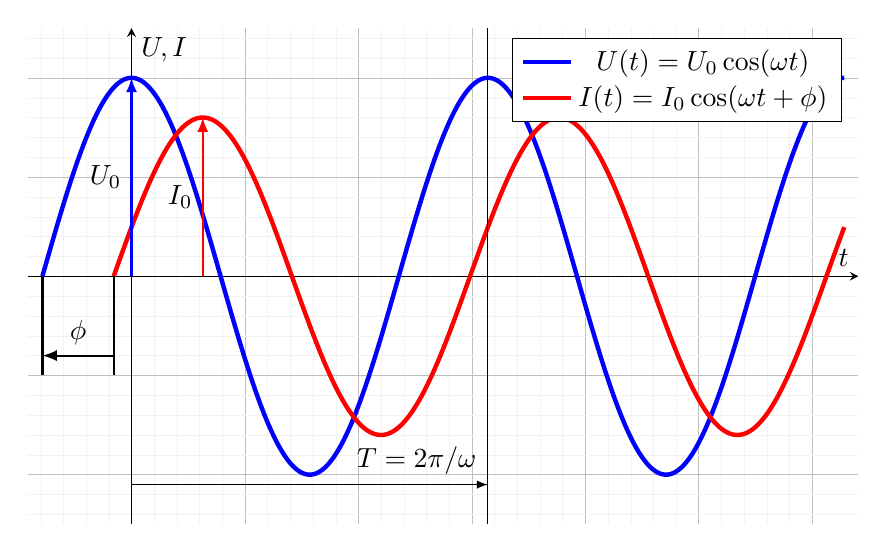
\begin{tikzpicture}
		\begin{axis}[%
				grid = both,
				major grid style={line width=.2pt,draw=gray!50},
				minor tick num = 4,
				minor grid style = {line width=.1pt,draw=gray!10},
				axis lines = middle,
				axis line style={-stealth},
				xlabel={$t$},
				ylabel={$U,I$},
				ytick style={draw=none},
				xtick style={draw=none},
				xticklabels={},yticklabels={},
				xmin = -pi/2,
				xmax = 4*pi,
				ymin = -1,
				ymax =  1,
				width=1\linewidth,
				height=0.65\linewidth,
				enlargelimits={abs=0.25},
			]
			\addplot+[ultra thick, samples=1000, blue, no marks, domain={-pi/2:4*pi}] {cos(deg(x))};
			\addplot+[ultra thick, samples=1000, red, no marks, domain={-(pi/2-0.4*pi):4*pi}] {4/5*cos(deg(x - 0.4*pi))};
			\draw[-latex, blue, thick] (axis cs:0,0) -- node[left, color = black] {$U_0$} (axis cs:0,1);
			\draw[-latex, red, thick] (axis cs:0.4*pi,0) -- node[left, color = black] {$I_0$} (axis cs:0.4*pi,4/5);
			\draw[thick] (axis cs:-pi/2,0) -- (axis cs:-pi/2,-0.5) (axis cs:-pi/2+0.4*pi,0) -- (axis cs:-pi/2+0.4*pi,-0.5);
			\draw[thick, latex-] (axis cs: -pi/2,-0.4) -- node[above] {$\phi$} (axis cs:-pi/2+0.4*pi,-0.4);
			\draw[] (axis cs: 2*pi,-1.25) -- (axis cs: 2*pi,1.25);
			\draw[-latex] (axis cs: 0,-1.05) -- node[above, pos=0.8] {$T = 2\pi/\omega$} (axis cs:2*pi,-1.05);
			\legend{$U(t) = U_0\cos(\omega t )$, $I(t) = I_0\cos(\omega t + \phi)$}
		\end{axis}
	\end{tikzpicture}
	\captionof{figure}{Графічне зображення синусоїдального змінного струму}
	\label{plt:sinusoidal_current}
\end{center}

\subsection{Діючі значення сили струму та напруги}

Окрім зазначених характеристик, змінний струм також характеризують діючим значенням $I_{\eff}$. \emph{Діюче значення змінного струму дорівнює такому значенню постійного струму, який за час, що дорівнює періоду виділяє на тому ж активному опорі таку ж кількість теплоти, що і даний змінний струм.}

Згідно закону Джоуля-Ленца, постійний струм величиною $I_{\eff}$  за час $T$ на резисторі $R$ виділить кількість теплоти $Q  = I_{\eff}^2 R T$, а змінний струм $I$ за період виділить кількість теплоти $Q = \int\limits_0^T I^2 R dt$.

Прирівнюючи ці два вирази отримаємо:
\[
	I_{\eff} = \sqrt{\frac1T\int\limits_0^T I^2 dt} = \sqrt{\left\langle I^2\right\rangle }.
\]
В цьому виразі під коренем стоїть величина, яка є середнім квадратичним значенням струму за період $T$. Для синусоїдального струму $I = I_0\cos(\omega t + \phi)$, як легко переконатись, ця величина дорівнює $\dfrac{I_0^2}{2}$, а тому, діюче значення струму дорівнюватиме:
\begin{equation}\label{Ieff}
	I_{\eff} = \frac{I_0}{\sqrt2}.
\end{equation}

Повторюючи аналогічні викладки для напруги можна отримати, вираз для діючого значення напруги:
\begin{equation}\label{Ueff}
	U_{\eff} = \frac{U_0}{\sqrt2}.
\end{equation}

Як видно з цих формул, діючі значення сили струму та напруги в $\sqrt2$ разів менше їх амплітудних значень.

\noindent\bigskip%
\begin{More}

	На шкалах вимірювальних приладів наносяться зазвичай саме діючі значення струму та напруги.

	Згідно даних, наведених в статті вікіпедії \href{https://uk.wikipedia.org/wiki/Побутова_електрична_мережа}{<<Побутова електрична мережа>>} наразі в Україні мережа має діюче значення напруги $230$~В  і частоту $50$~Гц.
\end{More}

\subsection{Послідовне коло змінного струму з активним, ємнісним та індуктивним опорами}

Будь-яке реальне електричне коло змінного струму містить активний опір (опір провідників, нагрівальних приладів, тощо), ємнісний опір (ємність провідників, конденсаторів) та індуктивний опір (обмотки електродвигунів, котушки електромагнітних приладів). Якщо до такого кола під’єднати двопроменевий осцилограф, то ми будемо спостерігати осцилограми коливань сили струму і напруги, які не збігаються за фазою (рис.~\ref{plt:sinusoidal_current}). Змінюючи індуктивність котушки (наприклад, вносячи залізне осердя) або ємність батареї конденсаторів, будемо спостерігати, що змінюється і різниця фаз.

\begin{wrapfigure}{L}{0.4\linewidth}
	\begin{tikzpicture}[every circuit symbol/.style={thick}]
		\draw[thick] (0,-2) coordinate (START) to [ac source={rotate=-90,info={left:$\mathcal{E}$}}] (0,2) -- ++(3,0) coordinate (A) to [resistor={info'={$R$}}] ++(0,-4/3) coordinate (B) to [inductor={info'={$L$}}] ++(0,-4/3) coordinate (C) to [capacitor={info'={$C$}}] ++(0,-4/3) coordinate (D)  -- (START)
		;
		\draw[red] (A) -- ++(1,0) (B) -- ++(1,0) (C) -- ++(1,0) (D) -- ++(1,0);
		\draw[<->, red] ([xshift=0.75cm]A) -- node[right, color=black] {$U_R$} ([xshift=0.75cm]B);
		\draw[<->, red] ([xshift=0.75cm]B) -- node[right, color=black] {$U_L$} ([xshift=0.75cm]C);
		\draw[<->, red] ([xshift=0.75cm]C) -- node[right, color=black] {$U_C$} ([xshift=0.75cm]D);
	\end{tikzpicture}
	\caption{Послідовне $RLC$-коло}
	\label{pic:S-RLC}
\end{wrapfigure}
Розглянемо електричне коло з активним, ємнісним та індуктивним навантаженнями, які з’єднані послідовно (рис.~\ref{pic:S-RLC}) (таке коло ще називають послідовним колом змінного струму).  З фізичної точки зору, така система є коливальним контуром, в якому здійснюватимуться вимушені гармонічні коливання під дією гармонічної напруги:
\begin{equation}\label{U_0}
	\mathcal{E} = \mathcal{E}_0\cos\omega t
\end{equation}

Згідно законів Ома, сума напруг на кожному елементі дорівнюватиме напрузі на генераторі:
\begin{equation}\label{ID_KL}
	U_R + U_L + U_C = IR + L\frac{dI}{dt} +  \frac{1}{C}\int I dt = \mathcal{E}_0\cos\omega t,
\end{equation}
де напруги на кожному елементі виражені через струм в колі, оскільки саме струм у випадку послідовного з'єднання буде однаковим на кожному елементі.

Отже, рівнянні~\eqref{ID_KL} є інтегро-диференціальним рівнянням відносно сили струму. У випадку \emph{встановлених} коливань, розв'язок цього рівняння будемо шукати у вигляді:
\begin{equation}\label{I}
	I = I_0\cos(\omega t + \phi),
\end{equation}
де $I_0$~--- амплітуда струму в колі (однакова на всіх елементах), $\phi$~--- зсув фаз між напругою та струмом.


\subsubsection{Метод комплексних амплітуд}

Розв'яжемо рівняння~\eqref{ID_KL} і знайдемо силу струму в колі, а також напруги на кожному з елементів кола. Одним із способів його розв'язку є \emph{метод комплексних амплітуд}.

\noindent\bigskip% 
\begin{More}
	Мати справу з гармонічними функціями не так просто, набагато легше працювати з експоненційними функціями, вони зручні при інтегруванні та диференціювання. Формула Ейлера
	\begin{equation*}
		e^{i\phi} = \cos\phi + i\sin\phi,
	\end{equation*}
	є ключовим виразом, який пов'язує гармонічні функції та комплекснозначну експоненту.

	Будь-яке комплексне число вигляду $z = a + ib$ можна представити у вигляді комплексної експоненти:
	\[
		z = |z|e^{\phi},
	\]
	де величина $|z| = \sqrt{a^2 + b^2}$ --- називається модулем комплексного числа $z$, а $\phi$~--- його фазою, яка визначається як $\tg\phi = \dfrac{b}{a}$, а його дійсна частина дорівнює $\Re{(z)} =|z|\cos\phi$.
\end{More}


Суть цього методу полягає в тому, що напругу слід представити як $\hat{U} = \hat{U}_0e^{i\omega t}$, а розв'язок шукати у вигляді $\hat{I} = \hat{I}_0e^{i\omega t}$, де величини $\hat{U}_0$  та $\hat{I}_0$ є комплексними амплітудами (<<шляпка>> над відповідною величиною означає, що вона є комплексною). Після розрахунків, для отримання вимірюваної величини, слід взяти дійсну частину отриманого комплексного виразу, попередньо представивши його у експоненційній формі: $I = |\hat{I}_0| \Re(e^{i(\omega t + \phi)})$. Такий метод називається \emph{методом комплексних амплітуд}. Скористаємось таким методом  і знайдемо розв'язок  шляхом підстановки $\hat{I} = \hat{I}_0e^{i\omega t}$ в рівняння~\eqref{ID_KL}:
\begin{equation}\label{Complex_Amplitudes}
	\hat{I}_0 R  + \hat{I}_0 i\omega L + \hat{I}_0 \frac{1}{i\omega C} = \hat{\mathcal{E}}_0.
\end{equation}
В останньому рівнянні зручно ввести величини $\hat{X}_L = i\omega L$ та $\hat{X}_C = \frac{1}{i\omega C}$, які називаються \emph{комплексними опорами} котушки та конденсатора, відповідно.

Отже, рівняння~\eqref{Complex_Amplitudes} можна представити у вигляді  $\hat{I}_0 \hat{Z} = \hat{\mathcal{E}}_0$, де $\hat{Z}$ називається \href{http://femto.com.ua/articles/part_1/1313.html}{\emph{імпедансом}} послідовного кола і визначається формулою:
\begin{equation}\label{total_impedance}
	\hat{Z} = R + \hat{X}_L + \hat{X}_C = R  +   i\left(  \omega L - \frac{1}{\omega C} \right) .
\end{equation}

\begin{More}

	Завдяки методу комплексних амплітуд, аналіз режимів в електричних колах суттєво спрощується. Рівняння електричного стану для кола змінного струму в комплексній формі подібні до рівнянь електричного стану для кіл постійного струму. Завдяки цьому, використання комплексних опорів, комплексних амплітуд струмів і напруг дозволяє записувати закони Ома таким же чином, як і в для постійних струмів.
\end{More}

Використовуючи рівняння~\eqref{Complex_Amplitudes}, бачимо, що комплексна амплітуда струму дорівнює:
\begin{equation}
	\hat{I}_0 = \frac{\hat{\mathcal{E}}_0}{R  +   i\left(  \omega L - \frac{1}{\omega C} \right)}.
\end{equation}

Виразимо останнє рівняння в експоненційній формі (позбавившись комплексності знаменника домноженням на комплексно-спряжену величину і скориставшись формулою Ейлера):
\begin{equation}
	\hat{I}_0 = \frac{\hat{\mathcal{E}}_0e^{i\phi}}{\sqrt{R^2  +   \left(  \omega L - \frac{1}{\omega C} \right)^2}},
\end{equation}
де $\phi$~--- є зсувом фаз між силою струму та напругою, і визначається співвідношенням
\begin{equation}\label{S-phase_shift}
	\tg\phi = \frac{\omega L - \frac{1}{\omega C}}{R},
\end{equation}
а модуль імпедансу
\begin{equation}
	Z = |\hat{Z}| = \sqrt{R^2  +   \left(  \omega L - \frac{1}{\omega C} \right)^2}.
\end{equation}
Отже, вираз для комплексного струму буде виглядати наступним чином (пам'ятаємо, що $\hat{\mathcal{E}}_0 = U_0$):
\begin{equation}\label{CI0}
	\hat{I}= \frac{\mathcal{E}_0}{Z}e^{i(\omega t + \phi)},
\end{equation}
а його дійсна частина буде розв'язком рівняння~\eqref{ID_KL}:
\begin{equation}
	I= \frac{\mathcal{E}_0}{Z}\cos(\omega t + \phi).
\end{equation}

Знайдемо тепер напруги на кожному з елементів кола з рівняння~\eqref{Complex_Amplitudes}
\begin{equation}\label{eq:S_sumU}
	\hat{U}_{0_R} + \hat{U}_{0_L} + \hat{U}_{0_C} = \hat{\mathcal{E}}_{0},
\end{equation}
де
\begin{equation*}
	\hat{U}_{0_R} = \hat{I}_{0} R, \quad \hat{U}_{0_L} = \hat{I}_{0} \hat{X}_L, \quad \hat{U}_{0_C} = \hat{I}_{0} \hat{X}_C , \quad \hat{\mathcal{E}}_{0} = \mathcal{E}_0.
\end{equation*}

Виразимо їх в експоненційній формі:
\begin{equation*}
	\hat{U}_{0_R} = I_0 R,  \quad \hat{U}_{0_L} = I_0\omega Le^{i\frac{\pi}{2}}, \quad \hat{U}_{0_C} = \frac{I_0}{\omega C}e^{-i \frac{\pi}{2}}, \quad \hat{\mathcal{E}}_{0} = \mathcal{E}_0.
\end{equation*}
З цих формул можна побачити зсуви фаз між напругами на елементах та силою струму в колі. Степінь комплексної експоненти нам говорить про те, що напруга $U_R$ на активному опорі  коливається в фазі із силою струму, напруга на котушці $U_L$ випереджує коивання струму на $\pi/2$, а напруга на конденсаторі навпаки, запізнюється по фазі на $\pi/2$, з цього також випливає, що напруги на конденсаторі і котушці коливаються в протифазі.

Модулі цих величин дають амплітудні значення напруг на елементах кола:
\begin{align}
	U_{0_R} & = I_0R =   \frac{\mathcal{E}_0 R}{\sqrt{R^2  +   \left(  \omega L - \frac{1}{\omega C} \right)^2}}, \label{U0R}       \\
	U_{0_L} & = I_0X_L = \frac{\mathcal{E}_0 \omega L}{\sqrt{R^2  +   \left(  \omega L - \frac{1}{\omega C} \right)^2}} \label{U0L} \\
	U_{0_C} & = I_0X_C = \frac{\mathcal{E}_0}{\omega C\sqrt{R^2  +   \left(  \omega L - \frac{1}{\omega C} \right)^2}}\label{U0C}.
\end{align}
Залежність амплітуд коливань від частоти генератора~\ref{plt:S-AFC} носить назву амплітудно-частотних характеристик (АЧХ), або резонансних кривих. Ширина АЧХ визначає найважливішу характеристику контуру --- його добротність.

%---------------------------------------------------------
\begin{center}
	\begin{minipage}{0.75\linewidth}
\begin{tikzpicture}%
[
declare function ={
L = 2;
C = 0.5;
R = 0.9;
U=15;
omegares = 1/sqrt(L*C);
Q = 1/R*sqrt(L/C);
UC(\x) = U/(x*C)/sqrt(R^2 + (x*L-1/(C*x))^2);
UL(\x) = U*(x*L)/sqrt(R^2 + (x*L-1/(C*x))^2);
UR(\x) = U*R/sqrt(R^2 + (x*L-1/(C*x))^2);
phi(\x) = rad(atan((x*L-1/(x*C))/R));
}
]
			\begin{groupplot}[group style={group size=1 by 2, vertical sep=2cm}]
				%---------------------------------------------------------
				\nextgroupplot[title={\small Амплітудно-частотна характеристики напруг},
					% === Налаштування сітки ===
					grid = both,
					major grid style={line width=.2pt,draw=gray!50},
					minor tick num = 4,
					minor grid style = {line width=.1pt,draw=gray!10},
					% === Налаштування положення координатних осей ===
					%axis x line=center, % top, center, bottom
					%axis y line=center, % left, center, right
					axis lines = middle,
					axis line style={-stealth},
					% === Підпис координатних осей ===
					xlabel={$\omega$},
					ylabel={$U$},
					extra x ticks={omegares},
					extra x tick labels={$\omega_0$},
					xticklabels={},
					yticklabels={},
					extra y ticks={U, Q*U},
					extra y tick labels={$\mathcal{E}_0$, $Q \mathcal{E}_0$},
					% === Положення підпису координатних осей ===
					xlabel style={below right},
					ylabel style={above left},
					xtick style={draw=none},
					ytick style={draw=none},
					% === Вибір підписів шкали для відображення ===
					xtick = {},
					ytick = {},
					% === Налаштування мінімальних та максимальних значень координат ===
					xmin = 0,
					xmax =  2*omegares,
					ymin = 0,
					ymax =  40,
					% === Налаштування розміру графіка ===
					width=1\linewidth,
					height=0.75\linewidth,
					]
				\addplot [ultra thick, samples = 1000, red, thick, domain=0.001:2*omegares] {UC(x)};
				\addplot [ultra thick,samples = 1000, blue, thick, domain=0.001:2*omegares] {UL(x)};
				\addplot [ultra thick,samples = 1000, green!50!black, thick, domain=0.001:2*omegares] {UR(x)};
				\legend{$U_{0_C}$,$U_{0_L}$,$U_{0_R}$}
				%---------------------------------------------------------
				\nextgroupplot[title={\small Фазово-частотна характеристика послідовного кола},
					% === Налаштування сітки ===
					grid = both,
					major grid style={line width=.2pt,draw=gray!50},
					minor tick num = 4,
					minor grid style = {line width=.1pt,draw=gray!10},
					% === Налаштування положення координатних осей ===
					axis lines = middle,
					yticklabel pos=right,
					axis line style={-stealth},
					% === Підпис координатних осей ===
					xlabel={$\omega$},
					ylabel={$\phi$},
					xticklabels={},
					yticklabels={},
					extra tick style={% changes for all extra ticks
							tick align=outside,
							grid style={dashed,draw=black}
						},
%					extra y tick style={
%	
%						},
					extra x ticks = {omegares},
					extra x tick labels={$\omega_0$},
					extra y ticks = {-pi/2,pi/2},
					ytick = {-pi/2,-pi/4,0,pi/4,pi/2},
					extra y tick labels={$-\frac{\pi}{2}$,$\frac{\pi}{2}$},
					xtick style={draw=none},
					ytick style={draw=none},
					% === Положення підпису координатних осей ===
					xlabel style={below right},
					ylabel style={above right},
					% === Налаштування мінімальних та максимальних значень координат ===
					xmin = 0,
					xmax =  2*omegares,
					ymin = -pi/2,
					ymax =  pi/2,
					% === Налаштування розміру графіка ===
					width=1\linewidth,
					height=0.4\linewidth,
				]
				\addplot [ultra thick,samples = 1000, green!50!black, thick, domain=0.01:2*omegares, name path global=ResCurve] {phi(x)};
				%---------------------------------------------------------
			\end{groupplot}
		\end{tikzpicture}
		\captionof{figure}{Амплітудно- і фазовочастотні характеристики послідовного кола}
		\label{plt:S-AFC}
	\end{minipage}
\end{center}
%---------------------------------------------------------


\begin{figure}[h!]\centering
	\begin{subfigure}[b]{0.30\linewidth}
		\centering
		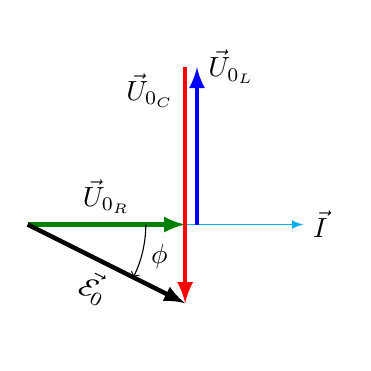
\begin{tikzpicture}[
				declare function = {
						UC = 3;
						UL = 2;
						UR = 2;
						DLC = (UL - UC);
						PhU = atan (DLC/UR);
					},
			]
			\path[use as bounding box] (0,-1.5) rectangle ++(4,4);
			\draw[-latex, cyan] (0,0) -- ++(3.5,0) node[right, color=black] {$\vec{I}$};
			\draw[-latex,  green!50!black,ultra thick] (0,0) -- ++(UR,0) node[above, pos=0.5, color=black] {$\vec{U}_{0_R}$};
			\draw[-latex,  blue, ultra thick] (UR+0.15,0) -- ++(0,UL) node[right, color=black] {$\vec{U}_{0_L}$};
			\draw[-latex,  red, ultra thick] (UR,UL) -- ++(0,-UC) node[left, color=black, pos=0.1] {$\vec{U}_{0_C}$};
			\draw[-latex,  black, ultra thick] (0,0) -- (PhU:{UR/cos(PhU)}) node[below, color=black, pos=0.5, sloped] {$\vec{\mathcal{E}}_{0}$} coordinate (U);
			%	\draw[dashed] (\UR,0) -- (U) (0,\DLC) -- (U);
			\draw[->] (0,0) ++(1.5,0) arc(0:PhU:1.5) node[pos=0.6, right] {$\phi$};
		\end{tikzpicture}
		\caption{$\omega < \omega_0$}
		\label{pic:S-vector_diagrams<}
	\end{subfigure}
	\begin{subfigure}[b]{0.30\linewidth}
		\centering
		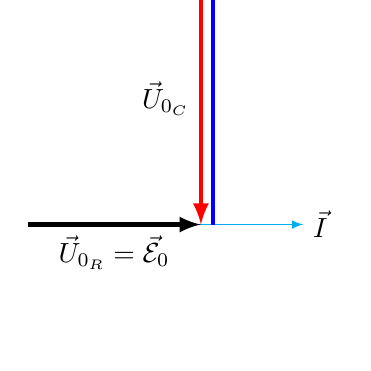
\begin{tikzpicture}[
				declare function = {
						UC = 3.2;
						UL = 3.2;
						UR = 2.2;
						DLC = (UL - UC);
						PhU = atan (DLC/UR);
					},
			]
			\path[use as bounding box] (0,-1.5) rectangle ++(4,4);
			\draw[-latex, cyan] (0,0) -- ++(3.5,0) node[right, color=black] {$\vec{I}$};
			\draw[-latex,  black,ultra thick] (0,0) -- ++({2/cos(atan(1/2.2)},0) node[below, pos=0.5, color=black] {$\vec{U}_{0_R} = \vec{\mathcal{E}}_{0}$};
			\draw[-latex,  blue, ultra thick] (UR+0.15,0) -- ++(0,UL) node[right, color=black] {$\vec{U}_{0_L}$};
			\draw[-latex,  red, ultra thick] (UR,UL) -- ++(0,-UC) node[left, color=black, pos=0.5] {$\vec{U}_{0_C}$};
		\end{tikzpicture}
		\caption{$\omega = \omega_0$}
		\label{pic:S-vector_diagrams=}
	\end{subfigure}
	\begin{subfigure}[b]{0.30\linewidth}
		\centering
		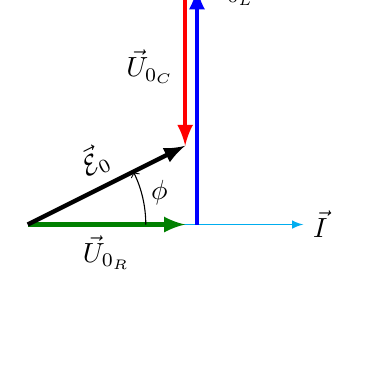
\begin{tikzpicture}[
				declare function = {
						UC = 2;
						UL = 3;
						UR = 2;
						DLC = (UL - UC);
						PhU = atan (DLC/UR);
					},
			]
			\path[use as bounding box] (0,-1.5) rectangle ++(4,4);
			\draw[-latex, cyan] (0,0) -- ++(3.5,0) node[right, color=black] {$\vec{I}$};
			\draw[-latex,  green!50!black,ultra thick] (0,0) -- ++(UR,0) node[below, pos=0.5, color=black] {$\vec{U}_{0_R}$};
			\draw[-latex,  blue, ultra thick] (UR+0.15,0) -- ++(0,UL) node[right, color=black] {$\vec{U}_{0_L}$};
			\draw[-latex,  red, ultra thick] (UR,UL) -- ++(0,-UC) node[left, color=black, pos=0.5] {$\vec{U}_{0_C}$};
			\draw[-latex,  black, ultra thick] (0,0) -- (PhU:{UR/cos(PhU)}) node[above, color=black, pos=0.5, sloped] {$\vec{\mathcal{E}}_{0}$} coordinate (U);
			%	\draw[dashed] (\UR,0) -- (U) (0,\DLC) -- (U);
			\draw[->] (0,0) ++(1.5,0) arc(0:PhU:1.5) node[pos=0.6, right] {$\phi$};
		\end{tikzpicture}
		\caption{$\omega > \omega_0$}
		\label{pic:S-vector_diagrams>}
	\end{subfigure}
	\caption{Векторні діаграми напруг для послідовного кола. \\ {\small \itshape Зсув фаз $\phi$ прийнято позначати стрілкою, яка напрямлена від вектора струму до вектора напруги}}
	\label{pic:S-vector_diagrams}
\end{figure}

Окрім методу комплексних амплітуд, синусоїдальні функції можна представляти також у вигляді векторів, які обертаються навколо вибраної осі з частотою $\omega$ і довжина яких дорівнює амплітуді відповідної величини. Такий метод називається \emph{методом векторних діаграм}. Векторні діаграми напруг для послідовного кола наведені на рис.~\ref{pic:S-vector_diagrams}.

\begin{More}

	Метод векторних діаграм і метод комплексних амплітуд --- методи опису синусоїдальних коливань, які мають свої переваги і недоліки
	\begin{enumerate}[label=$\checkmark$]
		\item Метод комплексних амплітуд більш потужний, оскільки природно включає в себе, складання і розв'язки систем рівнянь будь-якої складності, наприклад, для розгалужених кіл змінного струму, в той час як метод векторних діаграм в чистому вигляді все ж обмежений задачами, які передбачають графічні розрахунки.
		\item Метод векторних діаграм є більш наочним, а отже в деяких випадках потенційно більш надійний (дозволяє до певної міри уникнути грубих випадкових помилок, які можуть зустрічатися при абстрактних алгебраїчних обчисленнях) і дозволяє в деяких випадках досягти в якомусь сенсі більш глибокого розуміння задачі.
	\end{enumerate}
\end{More}


\subsubsection{Резонанс напруг в послідовному колі}

З формули~\eqref{CI0} видно, що за умови $X_L = X_C$, тобто:
\begin{equation}
	\omega L = \frac{1}{\omega C},
\end{equation}
яка задовольняється при співпадінні частоти генератора та власної частоти коливань електричного кола
\begin{equation}
	\omega = \omega_0 = \frac{1}{\sqrt{LC}},
\end{equation}
амплітуда сили струму в колі досягає свого максимального значення $I_0 = \dfrac{\mathcal{E}_0}{R}$, при цьому, напруга на резисторі також досягає свого максимального значення, що дорівнює амплітудному значенню напруги на генераторі $\mathcal{E}_0$, а напруги на конденсаторі і котушці стають однаковими:
\begin{align}
	U_{0_R}    & = \mathcal{E}_0                                                             \\
	U_{0_C}    & = U_{0_L} = \frac{1}{R} \sqrt{\frac{L}{C}} \mathcal{E}_0 = Q \mathcal{E}_0, \\
	U_{0_{LC}} & = U_{0_L} - U_{0_C} = 0 \label{ULC}
\end{align}
де $U_{0_{LC}}$~--- амплітуда напруги на $LC$-ділянці, а величина $Q$~--- називається \href{http://femto.com.ua/articles/part_1/1110.html}{\emph{добротністю контуру}}, її значення завжди більше одиниці, тому амплітуди напруг на котушці і конденсаторі перевищують  амплітудне значення напруги генератора в $Q$ разів (рис.~\ref{plt:S-AFC}). Тому таку явище в послідовному контурі називається \emph{резонансом напруг}.

Коли частота генератора менше частоти резонансної частоти кола, ємнісний опір переважає над індуктивним і контур представляє для генератора опір ємнісного характеру. Якщо частота генератора більше резонансної частоти кола, то індуктивний опір більше ємнісного і контур для генератора є опором індуктивного характеру. При резонансі опір кола є суто активним (рис.~\ref{plt:impedance_character}).

%---------------------------------------------------------
\begin{center}
	\begin{tikzpicture}[
			declare function={
					L  = 2;
					C  = 1.2e-3;
					R  = 80;
					omegares  = 1/sqrt(L*C);
					Q  = sqrt(L/C)/R;
					XL(\x) =\x*L;
					XC(\x) = 1/(C*\x) ;
				},
		]
		\begin{axis}[
				% === Налаштування сітки ===
				grid = both,
				major grid style={line width=.2pt,draw=gray!50},
				minor tick num = 4,
				minor grid style = {line width=.1pt,draw=gray!10},
				extra tick style={% changes for all extra ticks
						tick align=outside,
						grid style={dashed,draw=black}
					},
				extra x tick style={
						tick label style={
								xshift=5mm,
								/pgf/number format/.cd, fixed, fixed zerofill,
							}
					},
				% === Налаштування положення координатних осей ===
				axis lines = middle,
				axis line style={stealth-stealth},
				% === Підпис коор5динатних осей ===
				%				xticklabels={},
				xlabel={$\omega$},
				ylabel={},
				% === Положення підпису координатних осей ===
				ylabel style={above right},
				xticklabels={},
				yticklabels={},
				extra x ticks = {omegares},
				extra x tick labels = {$\omega_0$},
				ytick style={draw=none},
				xtick style={draw=none},
				% === Вибір підписів шкали для відображення ===
				xtick = {},
				ytick = {},
				legend style={at={(current axis.south east)},anchor=south east},
				% === Налаштування мінімальних та максимальних значень координат ===
				xmin = 6,
				xmax =  60,
				ymin = -150,
				ymax =  150,
				% === Налаштування розміру графіка ===
				width=1\linewidth,
				width=0.7\linewidth,
			]
			\addplot [ultra thick,samples = 500, blue, thick, domain=0.2*omegares:3*omegares,name path = UL]  {XL(x)};
			\addplot [ultra thick,samples = 500, red, thick, domain=0.2*omegares:3*omegares,name path = UC]  {-XC(x)};
			\addplot [ultra thick,samples = 500, green!50!black, thick, domain=0.2*omegares:3*omegares,name path = DU]  {XL(x)-XC(x)};
			\addplot [ultra thick,samples = 500, black, thick, domain=0.2*omegares:3*omegares,name path = DU]  {sqrt(R^2 + (XL(x)-XC(x))^2)};
			\legend{$X_L = \omega L$, $X_C = \frac{1}{\omega C}$, $Z_{LC} = X_L - X_C$, $Z = \sqrt{R^2 + (X_L - X_C)^2}$}
			\pgfplotsinvokeforeach{0.5,1,2}{
				\draw [-latex, blue, ultra thick] (axis cs:#1*omegares, 0) -- node[left] {$X_L$} (axis cs:#1*omegares, {XL(#1*omegares)});
				\draw [-latex, red, ultra thick] (axis cs:#1*omegares, 0) -- node[left] {$X_C$} (axis cs:#1*omegares, {-XC(#1*omegares)});
			}
			\draw [latex-latex, black] (axis cs:0.6*omegares, 0) -- node[fill=white] {$R$} (axis cs:0.6*omegares, {R});
			\draw [dashed] (axis cs:omegares, R) -- (axis cs:0.6*omegares, R);
		\end{axis}
	\end{tikzpicture}
	\captionof{figure}{Характер зміни імпедансу кола}
	\label{plt:impedance_character}
\end{center}

Добротність кола характеризує її якість. Більш високе значення цього показника відповідає більш вузькій смузі пропускання (що дуже бажано для багатьох схем). Якщо говорити простіше, то добротність є відношення енергії, накопиченої в реактивному опорі ланцюга, до енергії, що розсіюється активним опором цьому колі.

Добротність можна виразити дещо по іншому:

\begin{equation}
	Q = \frac{1}{R} \sqrt{\frac{L}{C}} = \frac{\omega_0 L}{R} = \frac{\omega_0}{2\Delta\omega}
\end{equation}

Ширина смуги частот на АЧХ $2\Delta\omega$ визначається на висоті $\dfrac1{\sqrt2}\approx 0.707$ від висоти максимуму (рис.~\ref{plt:I(o)}),  оскільки потужність і енергія пропорційні квадрату амплітуди коливань, то рівню $0.707$ відповідає точка половинної потужності, що дорівнює $P = I^2R$, $(0.707)^2 = 0.5$.

\noindent\bigskip%
\begin{More}

	З фізичної точки зору, при явищі резонансу напруг в колі відбувається обмін енергією між магнітним полем котушки і електричним полем конденсатора, при цьому обміну енергією між полем і джерелом живлення не відбувається.
\end{More}

\subsection{Еквівалентна схема реального послідовного контуру}

В реальному контурі конденсатор і котушка окрім ємнісного $X_L$ та індуктивного опорів $X_L$ також мають і активні опори $R_C$ та $R_L$. Активний опір конденсатора зумовлений струмами провідності в прошарку діелектрика, а котушки~--- матеріалом дротів.

%=========================================================
\begin{figure}[h!]\centering
	%---------------------------------------------------------
	\begin{minipage}[t]{0.3\linewidth}
		\centering
		\begin{tikzpicture}[thick, every circuit symbol/.style={thick}]
			\draw (0,0) node[contact] {} to [capacitor={info={$C$}}] ++(4,0) node[contact] {} (1,0) -- ++(0,-1) to [resistor={info={$R_C$}, color=red}] ++(2,0) -- ++ (0,1);
		\end{tikzpicture}
		\caption{Схема заміщення реального конденсатора}
		\label{pic:equiv_capacitor}
	\end{minipage}
	\quad%---------------------------------------------------------
	\begin{minipage}[t]{0.3\linewidth}
		\centering
		\begin{tikzpicture}[thick, every circuit symbol/.style={thick}]
			\draw (0,0) node[contact] {} to [resistor={info={$R_L$}, color=red}] ++(2,0) to [inductor={info={$L$}}] ++(2,0) node[contact] {};
			\path (0,0) -- ++(0,-1.05);
		\end{tikzpicture}
		\caption{Схема заміщення реальної котушки}
		\label{pic:equiv_inductor}
	\end{minipage}
	\quad%---------------------------------------------------------
	\begin{minipage}[t]{0.3\linewidth}
		\centering
		\begin{tikzpicture}[thick, every circuit symbol/.style={thick}]
			\draw (0,0) node[contact] {} to [resistor={info={$R_i$}, color=red}] ++(2,0) to [ac source={info={$\mathcal{E}$}}] ++(2,0) node[contact] {};
			\path (0,0) -- ++(0,-1.05);
		\end{tikzpicture}
		\caption{Схема заміщення реального генератора}
		\label{pic:equiv_ac_generator}
	\end{minipage}
	%---------------------------------------------------------
\end{figure}
%=========================================================



Окрім того, реальний генератор має свій внутрішній опір $R_i$. Тому, реальний конденсатор і котушка на схемах повинні бути представлені як реактивними, так і активними опорами, а для генератора треба врахувати наявність внутрішнього опору. Таке представлення називається \emph{схемою заміщення}, а вся схема --- \emph{еквівалентною}. Для досліджуваного інтервалу частот конденсатор зручно представляти паралельною схемою заміщення~\ref{pic:equiv_capacitor}, котушку послідовною~\ref{pic:equiv_inductor}, а герератор~\ref{pic:equiv_ac_generator}.

\begin{wrapfigure}{L}{0.45\linewidth}
	\centering
	\begin{tikzpicture}[thick, every circuit symbol/.style={thick}]
		\draw (0,-2) coordinate (START) to [resistor={info={$R_i$}, color=red}] ++(0,2) to [ac source={rotate=-90,info={left:$\mathcal{E}$}}] (0,2) to [resistor={info={$R_I$}}] coordinate (V1) ++(4,0) to [inductor={info={$L$}}] ++(0,-4/3) to [resistor={info={$R_{L}$}, color=red}] ++(0,-4/3) to [capacitor={info={$C$}}] ++(0,-4/3)  -- (START);
		\draw ([xshift=-0.75cm]V1) node [contact] {} -- ++(0,1) to [voltmeter] ++(1.5,0) -- ++(0,-1)  node [contact] {};
	\end{tikzpicture}
	\caption{Послідовне з'єднання елементів}
	\label{pic:equiv_serial_circuit}
\end{wrapfigure}
Оскільки, активний опір конденсатора вважатимемо нескінченно великим ($\approx 10^2$~МОм) в порівняні з величинами, як активних, так і реактивних (для досліджуваного частотного діапазону) опорів інших елементів кола, то еквівалентна схема при послідовного контуру буде мати вигляд, поданий на рис.~\ref{pic:equiv_serial_circuit}.

Під'єднавши клеми вольтметру до резистора $R_I$, можна безпосередньо виміряти залежність струму від частоти ($I_0 = \dfrac{U_{0_R}}{R_I}$). Аналітичний вигляд цієї залежності можна знайти методом комплексних амплітуд для схеми~\ref{pic:equiv_serial_circuit}:
\begin{equation}
	I_0 = \frac{\mathcal{E}_0}{\sqrt{(R_I + R_L + R_i)^2  +   \left(  \omega L - \frac{1}{\omega C} \right)^2}}.
\end{equation}

Завдяки наявності активного опору котушки, напруга на $LC$-ланцюжку при резонансі~\eqref{ULC} не дорівнюватиме нулю:
\[
	U_{0_{LC}} = U_{0_L} - U_{0_C} = I_0 R_L \approx 0,
\]
в чому можна переконатись, під'єднавши осцилограф при резонансі до цієї ділянки кола. Іншими словами, імпеданс цього ланцюжка стає найменшим і дорівнює його активному опору $R_L$ (який має порівняно невелику величину), а струм стає максимальним.



%---------------------------------------------------------
\begin{center}
	\begin{minipage}{0.75\linewidth}
		\begin{tikzpicture}
			\pgfset{fpu=true}
			\pgfmathsetmacro{\L}{2e-3}
			\pgfmathsetmacro{\C}{2.2e-6}
			\pgfmathsetmacro{\R}{10}
			\pgfmathsetmacro{\RL}{0.8}
			\pgfmathsetmacro{\Ri}{5}
			\pgfmathsetmacro{\U}{5}
			\pgfmathsetmacro{\omegares}{1/sqrt(\L*\C)}
			\pgfmathsetmacro{\Q}{sqrt(\L/\C)/\RL}
			\pgfmathsetmacro{\Imax}{\U/(\R + \Ri + \RL)}
			\pgfset{fpu=false}
			\begin{axis}[clip = false,
					% === Налаштування сітки ===
					grid = both,
					grid style={line width=.1pt, draw=gray!10},
					major grid style={line width=.2pt,draw=gray!50},
					minor tick num = 5,
					minor grid style = {line width=.1pt,draw=gray!10},
					% === Налаштування положення координатних осей ===
					%axis x line=center, % top, center, bottom
					%axis y line=center, % left, center, right
					axis lines = middle,
					axis line style={-stealth},
					% === Підпис координатних осей ===
					xticklabels={},
					%xlabel={$\omega$},
					ylabel={$\frac{I_{0}}{I_{\max}}$},
					xtick scale label code/.code={$\omega$, $\cdot 10^{#1}$},
					yticklabels={},
					xtick style={draw=none},
					ytick style={draw=none},
					% === Положення підпису координатних осей ===
					%				xlabel style={below right},
					ylabel style={above right},
					every x tick scale label/.style={at={(1,0)}, anchor = north},
					extra y ticks={1/sqrt(2), 1},
					extra x ticks={\omegares},
					extra y tick labels={$\frac{1}{\sqrt2}$, $1$},
					extra x tick labels={$\omega_0$},
					% === Вибір підписів шкали для відображення ===
					xtick = {},
					ytick = {},
					% === Налаштування мінімальних та максимальних значень координат ===
					xmin = 0,
					xmax =  3*\omegares,
					ymin = 0,
					ymax =  1,
					% === Налаштування розміру графіка ===
					width=1\linewidth,
					height=1\linewidth,
				]
				\addplot [ultra thick,samples = 500, green!50!black, thick, domain=0.1*\omegares:3*\omegares, name path global=ResCurve] {(\R + \RL + \Ri)/sqrt((\R + \RL + \Ri)^2 + (x*\L-1/(\C*x))^2};

				\path[name path=line] (axis cs:0, {1/sqrt(2)}) -- (axis cs:3*\omegares,{1/sqrt(2)});
				\draw [thick,
					dashed,
					name intersections={of=ResCurve and line},
				] (axis cs:0, {1/sqrt(2)}) -- (intersection-1) -- (intersection-2) (intersection-1) -- (intersection-1 |-0,0) node [below left] {$\omega_0 - \Delta\omega$} (intersection-2) -- (intersection-2 |-0,0) node [below right] {$\omega_0 + \Delta\omega$};
				\fill [white, draw=green!50!black, name intersections={of=ResCurve and line}] (intersection-1) circle (0.1cm) (intersection-2) circle (0.1cm);
			\end{axis}
		\end{tikzpicture}
		\captionof{figure}{Амплітудно-частотна характеристика напруги на резисторі послідовного контуру}
		\label{plt:I(o)}
	\end{minipage}
\end{center}
%---------------------------------------------------------

\noindent\bigskip%
\begin{More}

	Явище резонансу напруг використовують в \emph{електричних фільтрах}, наприклад якщо необхідно усунути з сигналу, що передається, складову струму певної частоти, то паралельно приймачу ставлять ланцюжок із сполучених послідовно конденсатора і котушки індуктивності, щоб струм резонансної частоти цього $LC$-ланцюжка замкнулося б через нього, і не потрапив до приймача. Тоді струми частоти далекою від резонансної частоти $LC$-ланцюжка будуть проходити в навантаження безперешкодно, і тільки близькі до резонансу по частоті струми --- знаходитимуть собі найкоротший шлях через $LC$-ланцюжок.

	Якщо необхідно пропустити тільки струм певної частоти, то $LC$-ланцюжок вмикають послідовно до приймача, тоді складові сигналу на резонансної частоті ланцюжка пройдуть до навантаження майже без втрат, а частоти далекі від резонансу стануть сильно ослаблені і можна сказати, що до навантаження зовсім не потраплять. Даний принцип можна застосувати до радіоприймачів, де коливальний контур налаштовують на прийом строго певної частоти потрібної радіостанції.

	Взагалі резонанс напруг в електротехніці є небажаним явищем, оскільки він викликає перенапруження і вихід з ладу обладнання. Як простий приклад можна привести довгу кабельну лінію, яка з якоїсь причини виявилася не підключеною до навантаження, але при цьому живиться від проміжного трансформатора. Така лінія з розподіленою ємністю і індуктивністю, якщо її резонансна частота співпаде з частотою мережі живлення, просто буде пробита і вийде з ладу.

	%	Крім того, при резонансі напруг слід бути обачним, і не чіпати контакти реактивних елементів контуру, оскільки навіть при низькому значенні амплітуди напруги генератора, при резонансі напруги на цих елементах перевищують її, що може бути небезпечним і завдати ураження організму.

\end{More}

\subsection{Паралельне коло змінного струму з активним, ємнісним та індуктивним опорами. Резонанс струмів}

\begin{wrapfigure}[]{L}{0.4\linewidth}
	\begin{tikzpicture}[every circuit symbol/.style={thick}]
		\draw[thick] (0,-2) coordinate (START) to [ac source={rotate=-90,info={left:$\mathcal{E}_0$}}] (0,2) coordinate (AC) -- ++(2,0) coordinate (A) to [resistor={info'={$R$}}] ++(0,-4) coordinate (B) -- (START)
		(A) -- ++(1.5,0) coordinate (A1) to [capacitor={info'={$C$}}] ++(0,-4) coordinate (B1) -- (B)
		(A1) -- ++(1.5,0) coordinate (A2) to [inductor={info'={$L$}}] ++(0,-4) -- (B1)
		;
		\draw[->,red, thick] ([xshift=0.25cm]AC) -- node[color=black, above] {$I$} ++(1,0);
		\draw[->,red, thick] ([yshift=-0.25cm]A) -- node[color=black, left] {$I_R$} ++(0,-1);
		\draw[->,red, thick] ([yshift=-0.25cm]A1) -- node[color=black, left] {$I_C$} ++(0,-1);
		\draw[<-,red, thick] ([yshift=-0.25cm]A2) -- node[color=black, left] {$I_L$} ++(0,-1);
	\end{tikzpicture}
	\caption{Паралельне $RLC$-коло}
	\label{pic:P-RLC}
\end{wrapfigure}
Розглянемо електричне коло, де котушка, конденсатор та резистор з'єднані паралельно (рис.~\ref{pic:P-RLC}). В цьому випадку, напруга на кожному елементі буде однакова, а загальний струм $I$ буде дорівнювати сумі струмів, що протікають через кожний з елементів:
\begin{equation}
	I = I_R + I_C +I_L.
\end{equation}

В цьому випадку також можна скористатись методом комплексних амплітуд і визначити струми на окремих елементах контуру та загальний струм в колі:

\begin{align}
	I_R & = \frac{\mathcal{E}_0}{R} \cos(\omega t), \label{IR}                                                                     \\
	I_C & = \mathcal{E}_0\omega C \cos (\omega t + \frac{\pi}{2}), \label{IC}                                                      \\
	I_L & = \frac{\mathcal{E}_0}{\omega L}\cos (\omega t - \frac{\pi}{2}), \label{IL}                                              \\
	I   & = \mathcal{E}_0\sqrt{\frac{1}{R^2}  +   \left(  \omega C - \frac{1}{\omega L} \right)^2} \cos(\omega t + \phi).\label{I}
\end{align}

Зсув фаз $\phi$ між напругою та загальним струмом у колі дорівнюватиме:
\begin{equation}\label{P-phase_shift}
	\tg\phi = \frac{\omega C - \frac{1}{\omega L}}{R}.
\end{equation}

З цих формул видно, що струм на резисторі $I_R$ коливається в фазі з напругою на генераторі, а його амплітуда не залежить від частоти, крім того, струми на конденсаторі $I_C$ і котушці $I_L$ коливаються в протифазі, і їх амплітуди залежать від частоти.

При частоті $\omega_0 = \dfrac{1}{\sqrt{CL}}$ амплітуда струму в колі досягає \emph{мінімального} значення $I_{0_{\min}} = I_{0_R}  = \dfrac{\mathcal{E}_0}{R}$, яка називається \emph{резонансною частотою}. При цьому струми на котушці та конденсаторі приймають однакові амплітудні значення $I_{0_C} = I_{0_L} = Q I_{0_{\min}}$, тобто перевищують силу струму в нерозгалудженій ділянці кола в $Q$ разів, при цьому контур поводить себе як активний опір ($\phi = 0$) величиною $Z = RQ^2$. Таке явище називається \emph{резонансом струмів} (рис.~\ref{plt:I(o)}).

%---------------------------------------------------------
\begin{center}
	\begin{minipage}{0.75\linewidth}
		\begin{tikzpicture}[
			declare function = {
					L  = 2;
					C  = 0.5;
					R  = 10;
					RL  = 0.1;
					U = 2;
					omegares  = 1/sqrt(L*C);
					Q  = sqrt(L/C)/R;
					I(\x) = U*sqrt( (1/R + RL/(RL^2+\x^2*L^2))^2 + (\x*C-L*\x/(RL^2 + L^2*\x^2))^2 );				
				}
			]
			%---------------------------------------------------------
			\begin{groupplot}[group style={group size=1 by 2, vertical sep=2cm}]
				%---------------------------------------------------------
				\nextgroupplot[title={\small Амплітудно-частотна характеристика паралельного кола},
					% === Налаштування сітки ===
					grid = both,
					grid style={line width=.1pt, draw=gray!10},
					major grid style={line width=.2pt,draw=gray!50},
					minor tick num = 5,
					minor grid style = {line width=.1pt,draw=gray!10},
					% === Налаштування положення координатних осей ===
					%axis x line=center, % top, center, bottom
					%axis y line=center, % left, center, right
					axis lines = middle,
					axis line style={-stealth},
					% === Підпис координатних осей ===
					xlabel={$\omega$},
					ylabel={$I$},
					xticklabels={},yticklabels={},
					xtick style={draw=none},
					ytick style={draw=none},
					extra tick style={% changes for all extra ticks
							tick align=outside,
							major grid style={dashed,draw=black}
						},
					extra x ticks = {omegares},
					extra x tick labels={$\omega_0$},
					extra y ticks = {I(omegares),U*omegares*C},
					extra y tick labels={$I_0$, $I_0/Q$},
					% === Положення підпису координатних осей ===
					xlabel style={below right},
					ylabel style={above left},
					% === Вибір підписів шкали для відображення ===
					xtick = {},
					ytick = {},
					% === Налаштування мінімальних та максимальних значень координат ===
					xmin = 0,
					xmax =  2,
					ymin = 0,
					ymax =  4,
					% === Налаштування розміру графіка ===
					width=1\linewidth,
					height=0.96\linewidth,
				]
				\addplot [ultra thick,samples = 500, green!50!black, thick,domain=0:2, restrict y to domain=0:4, name path global=ResCurve] {I(x)};
				\addplot [ultra thick,samples = 500, red, thick, domain=0:2, restrict y to domain=0:4] {U*x*C};
				\addplot [ultra thick,samples = 500, blue, thick, domain=0:2, restrict y to domain=0:4] {U/sqrt(x^2*L^2 + RL^2)};
				\legend{$I_0$, $I_{0_C}$, $I_{0_L}$}
				%---------------------------------------------------------
				\nextgroupplot[title={\small Фазово-частотна характеристика паралельного кола},
					% === Налаштування сітки ===
					grid = both,
					grid style={line width=.1pt, draw=gray!10},
					major grid style={line width=.2pt,draw=gray!50},
					minor tick num = 4,
					minor grid style = {line width=.1pt,draw=gray!10},
					% === Налаштування положення координатних осей ===
					axis lines = middle,
					yticklabel pos=right,
					axis line style={-stealth},
					% === Підпис координатних осей ===
					xlabel={$\omega$},
					ylabel={$\phi$},
					xticklabels={},
					yticklabels={},
					extra tick style={% changes for all extra ticks
							tick align=outside,
							grid style={dashed,draw=black}
						},
%					extra y tick style={
%	
%						},
					extra x ticks = {omegares},
					extra x tick labels={$\omega_0$},
					extra y ticks = {-pi/2,pi/2},
					ytick = {-pi/2,-pi/4,0,pi/4,pi/2},
					extra y tick labels={$-\frac{\pi}{2}$,$\frac{\pi}{2}$},
					xtick style={draw=none},
					ytick style={draw=none},
					% === Положення підпису координатних осей ===
					xlabel style={below right},
					ylabel style={above right},
					% === Налаштування мінімальних та максимальних значень координат ===
					xmin = 0,
					xmax =  2*omegares,
					ymin = -pi/2,
					ymax =  pi/2,
					% === Налаштування розміру графіка ===
					width=1\linewidth,
					height=0.4\linewidth,
				]
				\addplot [ultra thick,samples = 1000, green!50!black, thick, domain=0.01:2*omegares, name path global=ResCurve] {rad(-atan((x*L-1/(x*C))/RL))};
				%---------------------------------------------------------
			\end{groupplot}
		\end{tikzpicture}
		\captionof{figure}{Амплітудно- і фазовочастотні характеристики паралельного кола}
		\label{plt:P-AFC}
	\end{minipage}
\end{center}
%---------------------------------------------------------

\begin{figure}[h!]\centering
	\begin{subfigure}[b]{0.30\linewidth}
		\centering
		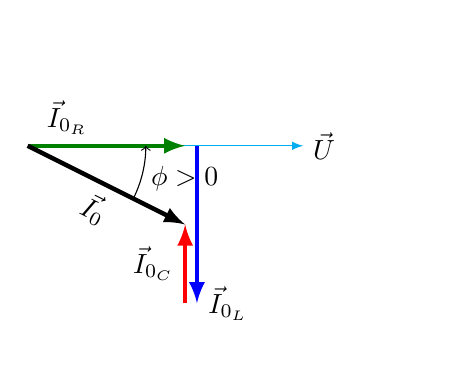
\begin{tikzpicture}[
				declare function = {
						IC = 1;
						IL = 2;
						IR = 2;
						DLC = (IL - IC);
						PhI = -atan(DLC/IR);
					},
			]
			\path[use as bounding box] (0,1.5) rectangle ++(5,-4);
			\draw[-latex, cyan] (0,0) -- ++(3.5,0) node[right, color=black] {$\vec{U}$};
			\draw[-latex,  green!50!black,ultra thick] (0,0) -- ++(IR,0) node[above, pos=0.25, color=black] {$\vec{I}_{0_R}$};
			\draw[-latex,  blue, ultra thick] (IR+0.15,0) -- ++(0,-IL) node[right, color=black] {$\vec{I}_{0_L}$};
			\draw[-latex,  red, ultra thick] (IR,-IL) -- ++(0,IC) node[left, color=black, pos=0.5] {$\vec{I}_{0_C}$};
			\draw[-latex,  black, ultra thick] (0,0) -- (PhI:{IR/cos(PhI)}) node[below, color=black, pos=0.5, sloped] {$\vec{I}_{0}$} coordinate (I);
			\draw[<-] (0,0) ++(1.5,0) arc(0:PhI:1.5) node[pos=0.6, right] {$\phi > 0$};
		\end{tikzpicture}
		\caption{$\omega < \omega_0$}
		\label{pic:P-vector_diagrams<}
	\end{subfigure}
	\begin{subfigure}[b]{0.30\linewidth}
		\centering
		\begin{tikzpicture}[
				declare function = {
						IC = 1.5;
						IL = 1.5;
						IR = 2;
						DLC = (IL - IC);
						PhI = -atan(DLC/IR);
					},
			]
			\path[use as bounding box] (0,1.5) rectangle ++(5,-4);
			\draw[-latex, cyan] (0,0) -- ++(3.5,0) node[right, color=black] {$\vec{U}$};
			\draw[-latex,  green!50!black,ultra thick] (0,0) -- ++(IR,0) node[above, pos=0.5, color=black] {$\vec{I}_{0_R} = \vec{I}_{0}$};
			\draw[-latex,  blue, ultra thick] (IR+0.15,0) -- ++(0,-IL) node[right, color=black] {$\vec{I}_{0_L}$};
			\draw[-latex,  red, ultra thick] (IR,-IL) -- ++(0,IC) node[left, color=black, pos=0.2] {$\vec{I}_{0_C}$};
		\end{tikzpicture}
		\caption{$\omega = \omega_0$}
		\label{pic:P-vector_diagrams=}
	\end{subfigure}
	\begin{subfigure}[b]{0.30\linewidth}
		\centering
		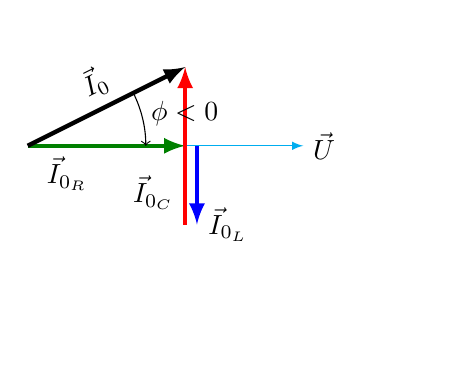
\begin{tikzpicture}[
				declare function = {
						IC = 2;
						IL = 1;
						IR = 2;
						DLC = (IL - IC);
						PhI = -atan(DLC/IR);
					},
			]
			\path[use as bounding box] (0,1.5) rectangle ++(5,-4);
			\draw[-latex, cyan] (0,0) -- ++(3.5,0) node[right, color=black] {$\vec{U}$};
			\draw[-latex,  green!50!black,ultra thick] (0,0) -- ++(IR,0) node[below, pos=0.25, color=black] {$\vec{I}_{0_R}$};
			\draw[-latex,  blue, ultra thick] (IR+0.15,0) -- ++(0,-IL) node[right, color=black] {$\vec{I}_{0_L}$};
			\draw[-latex,  red, ultra thick] (IR,-IL) -- ++(0,IC) node[left, color=black, pos=0.2] {$\vec{I}_{0_C}$};
			\draw[-latex,  black, ultra thick] (0,0) -- (PhI:{IR/cos(PhI)}) node[above, color=black, pos=0.5, sloped] {$\vec{I}_{0}$} coordinate (I);
			\draw[<-] (0,0) ++(1.5,0) arc(0:PhI:1.5) node[pos=0.6, right] {$\phi < 0$};
		\end{tikzpicture}
		\caption{$\omega > \omega_0$}
		\label{pic:P-vector_diagrams>}
	\end{subfigure}
	\caption{Векторні діаграми струмів для паралельного кола}
	\label{pic:P-vector_diagrams}
\end{figure}
%---------------------------------------------------------

При виникненні резонансу струму в колі його  реактивна складова стає рівною нулю, і як наслідок, повна провідність кола знижується до мінімального значення. Тому при постійній напрузі на затискачах даної схеми струм в нерозгалудженій частині  стає мінімальний, на відміну від резонансу напруги, коли струм максимальний. При цьому сумарний струм даному колі буде дорівнює векторній сумі всіх трьох струмів, два з яких (а саме $I_L$ і $I_C$) знаходяться в протифазі. Саме з --- за того, що $I_L$ і $I_C$ знаходяться в протифазі в $LC$-ділянці починає протікати струм, який при резонансі може значно перевищувати сумарний струм $I$.

\noindent\bigskip%
\begin{More}

	Явище резонансу струмів використовується в прийомних пристроях для виділення електромагнітного сигналу в вузькому спектральному інтервалі частот поблизу резонансної частоти.

	В індукційних печах паралельно котушці, що створює змінне магнітне поле, підключають ємність. Якщо умови резонансу виконуються, то струм в котушці збільшується в багато разів, а струм в підвідних проводах при цьому відносно невеликий.
\end{More}

\subsection{Еквівалентна схема паралельного контуру}

Для аналізу властивостей реального паралельного контуру також використаємо схеми заміщення для його елементів. які наведені на рис.~\ref{pic:equiv_capacitor}, \ref{pic:equiv_inductor} та \ref{pic:equiv_ac_generator}.


\begin{wrapfigure}{L}{0.45\linewidth}
	\centering
	\begin{tikzpicture}[thick, every circuit symbol/.style={thick}]
		\draw (0,-2) coordinate (START) to [resistor={info={$R_i$}, color=red}] ++(0,2) to [ac source={rotate=-90,info={left:$\mathcal{E}$}}] (0,2) to[resistor={info={$R_I$}}] ++(2,0)  coordinate (V1) -- ++(2,0) -- ++(0,-3/4) node [contact] {}  coordinate (C)

		(C) -- ++(1,0) to [resistor={info={$R_L$}, color = red}]  ++(0,-5/4) to [inductor={info={$L$}}] ++(0,-5/4)   --  ++(-1,0) coordinate (B) node [contact] {}
		(C) -- ++(-1,0) to [capacitor={info={$C$}}] ++(0,-10/4)  -- ++(1,0)
		(B) -- ++(0,-3/4)  -- (START);
		\draw (C) to [resistor={info={$R$}}] (B);
		\draw[<->, red] (V1) -- node[color = black, fill=white] {$U_{0_{RLC}}$} ++(0,-4);
	\end{tikzpicture}
	\caption{Паралельне з'єднання елементів з урахуванням заміщення}
	\label{pic:equiv_paralel_circuit}
\end{wrapfigure}
Знову ж, активний опір будемо вважати набагато більним за опрори інших елементів для досліджуваного інтервалу частот, а тому еквівалентна схема буде мати вигляд, поданий на рис.~\ref{pic:equiv_paralel_circuit}.

Під'єднавши клеми вольтметру до паралельного контуру, можна безпосередньо виміряти залежність напруги на контурі від частоти. Знайдемо аналітичний вигляд цієї залежності методом комплексних амплітуд. Так, згідно закону Ома:

\begin{equation}\label{Urlc}
	\hat{U}_{0_{RLC}} = \hat{\mathcal{E}}_0 - \hat{I}_0 (R_i + R_I),
\end{equation}
де $\hat{U}_0$~--- амплітуда ЕРС генератора, а $U_{0_{RLC}}$~--- напруга на паралельному контурі.

Оскільки при резонансі струм в колі падає до значення, яке близьке до нуля, то згідно~\eqref{Urlc} напруга має зростати.

Залежність напруги $U_{0_{RLC}}$~\eqref{Urlc}  та сили струму $I_0$ в колі побудована на рис.~\ref{plt:P-AFC-URLC}.

\begin{center}
	\begin{minipage}{0.75\linewidth}
		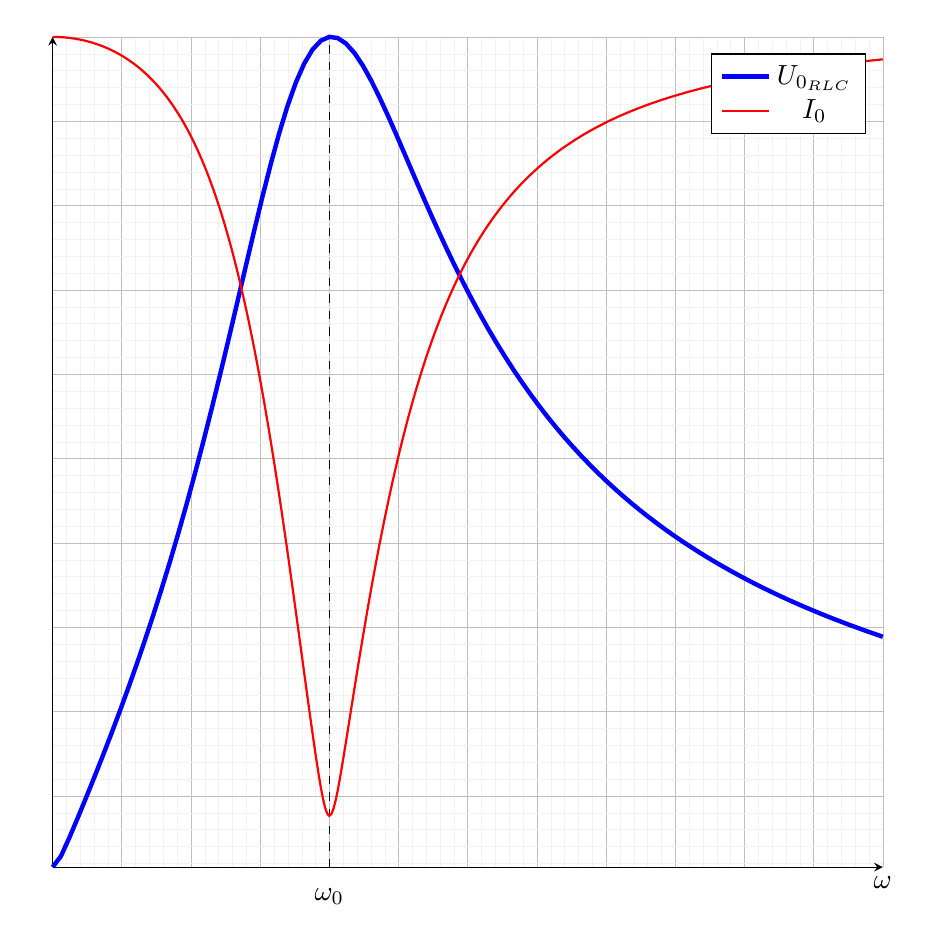
\begin{tikzpicture}[%/pgf/foreach/parse=true,
				declare function = {
						L = 2e-0;
						C = 1.2e-3;
						R = 1e3;
						RI = 50;
						RL = 0.8;
						Ri = 5 ;
						E = 10;
						omegares = 1/sqrt(L*C);
						a(\x) = 1/R + RL/(RL^2 + \x^2*L^2);
						b(\x) = \x*C - \x*L/(RL^2 + \x^2*L^2);
						c(\x) = (RI + Ri) + a(\x)/(a(\x)^2 + b(\x)^2);
						d(\x) =  b(\x)/(a(\x)^2 + b(\x)^2);
						g(\x) = c(\x)^2 + d(\x)^2;
						I(\x) = E/sqrt(g(\x));
						Imin = I(omegares);
						U(\x) = E*sqrt( (1- (Ri+ RI)*c(\x)/g(\x))^2 + ((Ri+ RI)*d(\x)/g(\x))^2 );
						Umax = U(omegares);
					},
			]
			\begin{axis}[clip = false,
					% === Налаштування сітки ===
					grid = both,
					grid style={line width=.1pt, draw=gray!10},
					major grid style={line width=.2pt,draw=gray!50},
					minor tick num = 4,
					minor grid style = {line width=.1pt,draw=gray!10},
					% === Налаштування положення координатних осей ===
					axis lines = middle,
					axis line style={-stealth},
					% === Підпис координатних осей ===
					%				xticklabels={},
					xlabel={$\omega$},
					%				ylabel={$\frac{U_{0_{RLC}}}{U_{0_{\max}}}$},
					% === Положення підпису координатних осей ===
					ylabel style={left},
					xlabel style={below},
					extra tick style={% changes for all extra ticks
							tick align=outside,
							major grid style={dashed,draw=black}
						},
					extra x tick style={
							major tick style={
								},
							tick label style={
									/pgf/number format/.cd, fixed, fixed zerofill,
									precision=2,
								}
						},
					xtick style={draw=none},
					ytick style={draw=none},
					xticklabels={},
					yticklabels={},
					extra x ticks={omegares},
					extra x tick labels={$\omega_0$},
					%				extra y ticks={(E - I(0)*(Ri + RI))/Umax},
					%				extra y tick labels={$\frac{\mathcal{E} - I(0)\cdot R_i}{U_{\max}}$},
					% === Вибір підписів шкали для відображення ===
					xtick ={0,
						0.25*omegares, 
						0.5*omegares,
						0.75*omegares,
						1*omegares,
						1.25*omegares,
						1.5*omegares,
						1.75*omegares,
						2*omegares,
						2.25*omegares,
						2.5*omegares,
						2.75*omegares,
						3*omegares},
					ytick = {},
					% === Налаштування мінімальних та максимальних значень координат ===
					xmin = 0*omegares,
					xmax = 3*omegares,
					ymin = {(E - I(0)*(Ri + RI))/Umax},
					ymax =  1,
					% === Налаштування розміру графіка ===
					width=1\linewidth,
					height=1\linewidth,
				]

				\addplot [ultra thick,samples = 100, domain=0*omegares:3*omegares, blue] {U(x)/Umax};
				\addplot [ultra thick,samples = 400, thick, domain=0*omegares:3*omegares, red] {I(x)/I(0)};
				\legend{$U_{0_{RLC}}$, $I_0$}
				%			\legend{$\frac{U_{0_{RLC}}}{U_{0_{\max}}}$, $\frac{I_0(\omega)}{I_0(\omega \to 0)}$}	
			\end{axis}
		\end{tikzpicture}
		\captionof{figure}{Амплітудно-частотна характеристика напруги на $RLC$-ділянці та загального струму в колі}
		\label{plt:P-AFC-URLC}
	\end{minipage}
\end{center}

У випадку $R_L \ll \omega L$ всі співвідношення при резонансі носять наближений характер:
\begin{equation*}
	\omega_{\mathrm{res}} \approx \omega_0 = \frac{1}{\sqrt{CL}},   \quad  I_{0_C}   \approx I_{0_L}, \quad 	I_0 \approx Q I_{0_C}, 	\quad \phi   \approx 0.
\end{equation*}

\section{Методика дослідження}

\subsection{Опис методики дослідження}


На коливальний контур подають синусоїдальну зовнішню напругу з контрольованою частотою $\omega = 2\pi \nu$, вимірюють залежність струму від частоти.

У випадку послідовного з'єднання конденсатора і котушки індуктивності на резонансній частоті $\omega_0$ повинні спостерігатися максимум амплітуди струму (напруги на резисторі $R_I$). При паралельному з'єднанні конденсатора і котушки резонанс в контурі виявляють по мінімальній напрузі на резисторі $R_I$, або по максимальній напрузі на конденсаторі і котушці.

Для визначення струму в колі, вимірюють напругу на резисторі $R_I$ за допомогою вольтметру універсального \tcbox{\sc{В7-16А}}, для вимірювань напруги на $LC$-ланцюжку використовується осцилограф \tcbox{\sc{C1-83}}.

Для дослідження явища резонансу використовують електричні кола, наведені на рис.~\ref{pic:serial_circuit} та \ref{pic:paralel_circuit}. Коло з послідовно з'єднаними елементами $L$ і $C$ (рис.~\ref{pic:serial_circuit}) призначене для вивчення резонансу напруг, а коло з паралельним з'єднанням  $L$ і $C$ (рис.~~\ref{pic:paralel_circuit}) --- для резонансу струмів.

%=========================================================
\begin{figure}[h!]\centering
	%---------------------------------------------------------
	\begin{minipage}[t]{0.45\linewidth}
		\centering
		\begin{tikzpicture}[thick, every circuit symbol/.style={thick}]
			%			\draw[blue, fill=blue!20] (1,1.5) rectangle ++(2,2);
			\draw[red, fill=red!20] (-0.7,-1.6) rectangle ++(1.2,3.1);
			\draw (0,-2) coordinate (START) to [resistor={info={$R_i$}, color=red}] ++(0,2) to [ac source={rotate=-90,info={left:$\mathcal{E}$}}] ++(0,2) to [resistor={info={$R_I$}}] coordinate (V1) ++(4,0) to [resistor={info={$R_{L}$}, color=red}] ++(0,-4/3) to [inductor={info={$L$}}] ++(0,-4/3) to [capacitor={info={$C$}}] ++(0,-4/3)  -- (START)
			;
			\draw ([xshift=-0.75cm]V1) node [contact] {} -- ++(0,1) to [voltmeter] ++(1.5,0) -- ++(0,-1)  node [contact] {};
		\end{tikzpicture}
		\caption{Послідовне з'єднання елементів}
		\label{pic:serial_circuit}
	\end{minipage}
	\quad%---------------------------------------------------------
	\begin{minipage}[t]{0.47\linewidth}
		\centering
		\begin{tikzpicture}[thick, every circuit symbol/.style={thick}]
			\draw[red, fill=red!20] (-0.7,-1.6) rectangle ++(1.2,3.1);
			\draw (0,-2) coordinate (START) to [resistor={info={$R_i$}, color=red}] ++(0,2) to [ac source={rotate=-90,info={left:$\mathcal{E}$}}] (0,2) to [resistor={info={$R_I$}}] ++(2,0)  coordinate (V1) -- ++(2,0) -- ++(0,-3/4) node [contact] {}  coordinate (C)

			(C) -- ++(1,0) to [resistor={info={$R_L$}, color = red}]  ++(0,-5/4) to [inductor={info={$L$}}] ++(0,-5/4)   --  ++(-1,0) coordinate (B) node [contact] {}
			(C) -- ++(-1,0) to [capacitor={info={$C$}}] ++(0,-10/4)  -- ++(1,0)
			(B) -- ++(0,-3/4)  -- (START);
			\draw (C) to [resistor={info={$R$}}] (B);
			\draw[] (V1) node [contact] {} to[voltmeter] ++(0,-4) node [contact] {};
			\draw (V1) node [contact] {} -- ++(0,1) to [voltmeter] ++(-2,0) -- ++(0,-1)  node [contact] {};
		\end{tikzpicture}
		\caption{Паралельне з'єднання елементів}
		\label{pic:paralel_circuit}
	\end{minipage}
	%---------------------------------------------------------
\end{figure}

%=========================================================
\section{Підготовка до рботи}

\subsection*{Початкове положення органів до включення в мережу}

\subsubsection*{Генератор}

\begin{enumerate}
	\item Перемикач \tcbox{\sc{ОСЛАБЛЕНИЕ dB}} --- в положенні \tcbox{\sc{0}} ;
	\item тумблер \tcbox{\sc{ВНУТР. 600 Ω}} --- в положенні \tcbox{\sc{ВКЛ.}};
	\item перемикач \tcbox{\sc{ВНЕШ. НАГРУЗКА Ω}} --- в положенні \tcbox{\sc{5}};
	\item увімкнена одна з кнопок перемикача \tcbox{\sc{МНОЖИ­ТЕЛЬ ЧАСТОТЫ}};
	\item ручка \tcbox{\sc{РЕГ. ВЫХОДА}} знаходиться в середньому положенні;
	\item ручки \tcbox{\sc{ЧАСТОТА Hz}} --- в довільному положенні;
	\item тумблер \tcbox{\sc{ШКАЛА ВОЛЬТМЕТРА}} --- в положенні \tcbox{\sc{63,2 V}}.
\end{enumerate}

\subsubsection*{Вольтметр \tcbox{\sc{В7-16А}} та осцилограф \tcbox{\sc{C1-83}}}

\begin{enumerate}
	\item На вольтметрі \tcbox{\sc{В7-16А}} встановіть ручку \tcbox{\sc{ПРЕДЕЛ ИЗМЕРЕНИЯ}} в положення \tcbox{\sc{10}}, ручку \tcbox{\sc{РОД РАБОТЫ}}  в положення \tcbox{\sc{$\sim$ U}}. Для підключення вольтметра використовуйте чорну клему входу  \tcbox{\sc{0}} та білу клему  \tcbox{\sc{$\simeq$ 100 V}}. Також врахуйте, що вхідний опір вольтметра в режимі вимірювання змінного струму становить всього $1$~МОм, тому не рекомендується ним вимірювати напругу на паралельному $RLC$~колі, натомість використовуйте осцилограф.
	\item На осцилографі \tcbox{\sc{C1-83}} встановіть ручку \tcbox{\sc{V/ДЕЛ}} на \tcbox{\sc{Канал I}} в положення \tcbox{\sc{5}}.
\end{enumerate}

\subsection*{Положення органів після включення приладів в мережу}

\begin{enumerate}
	\item Ручкою \tcbox{\sc{РЕГ. ВЫХОДА}} на генераторі \tcbox{\sc{ГЗ-56/1}} встановіть максимальну напругу генератора (дивіться на шкалу вольтметра генератора).
\end{enumerate}

\section{Завдання}

\begin{enumerate}
	\item Визначте внутрішній активний опір генератора $R_i$.
	\item Зберіть електричне коло за схемами
	      \begin{enumerate}[label=\alph*)]
		      \item послідовного з'єднання~\ref{pic:serial_circuit} ($R_I = 10$~Ом; $50$~Ом, $C = 1.2$~мкФ);
		      \item паралельного з'єднання~\ref{pic:paralel_circuit} ($R_I = 10$~Ом, $R = 1$~кОм; $2.2$~кОм та $C = 1.2$~мкФ). В якості вольтметра на резисторі $R_I$ використовуйте прилад \tcbox{\sc{В7-16А}}, в якості вольтметра для $RLC$~ланцюжка -- осцилограф.
	      \end{enumerate}
	      {\small\itshape На схемах в червоному прямокутнику показано генератор змінної напруги зі своїм внутрішнім опором $R_i$, в синьому прямокутнику показано під'єднання вольтметру до резистора відомого опору для вимірювання сили струму в колі.}
	\item Переконайтесь за допомогою осцилографа, що \emph{при резонансі} у випадку
	      \begin{enumerate}[label=\alph*)]
		      \item послідовного контуру~\ref{pic:serial_circuit}  напруга на $LC$-ділянці досягає мінімального значення;
		      \item паралельного контуру~\ref{pic:paralel_circuit} струм в колі досягає мінімального значення (для цього заміряйте напругу на резисторі $R_I$).
	      \end{enumerate}
	\item Зніміть амплітудно-частотні характеристики в досліджуваному колі для кіл з різними опорами $R_I$ ($R$).
	\item Визначте добротність електричного кола та резонансну частоту.
	\item Розрахуйте загальний опір втрат.
	\item Розрахуйте теоретично добротність електричного кола та резонансну частоту враховуючи отримане значення опору втрат, та порівняйте їх з експериментальними значеннями.
	\item Оцініть похибки вимірювання.
\end{enumerate}

\section*{Контрольні запитання}

\begin{enumerate}
	\item Які струм називається квазістаціонарним? Що розуміють під терміном <<змінний струм>>?
	\item Поясніть метод комплексних амплітуд та сформулюйте на їх основі правила Кірхгофа для кіл змінного струму.
	\item Що таке імпеданс?
	\item Що таке активний та реактивний опори?
	\item Що таке добротність електричного кола?
	\item Опишіть явища резонансу напруг та струмів в колах змінного струму.
\end{enumerate}

\end{document}
